
%%%%%%%%%%%%%%%%%%%%%%% file typeinst.tex %%%%%%%%%%%%%%%%%%%%%%%%%
%
% Template author: Mauricio Matamoros
% Updated: July 3, 2017
% Contact: mauricio@robocupathome.org
%
% This is the LaTeX source for the TDPTemplate using
% the LaTeX document class 'llncs.cls' Springer LNAI format
% used in the RoboCup Symposium submissions.
% http://www.springer.com/computer/lncs?SGWID=0-164-6-793341-0
%
% It may be used as a template for your own TDP - copy it
% to a new file with a new name and use it as the basis
% for your Team Description Paper
%
% NB: the document class 'llncs' has its own and detailed documentation, see
% ftp://ftp.springer.de/data/pubftp/pub/tex/latex/llncs/latex2e/llncsdoc.pdf
%
% Remark: Last page with specs won't be included in Camera ready TDP's.
%
%%%%%%%%%%%%%%%%%%%%%%%%%%%%%%%%%%%%%%%%%%%%%%%%%%%%%%%%%%%%%%%%%%%
%
% TU/e update: 27 oct 2017 - HvR

\documentclass[runningheads,a4paper]{llncs}
%\usepackage[left=48mm,right=46mm]{geometry}
%\usepackage[left=32mm,right=31mm]{geometry}

\usepackage[utf8]{inputenc}
\usepackage{amssymb}
\setcounter{tocdepth}{3}
\usepackage{url}
\usepackage{float}
\usepackage{amsmath}
\usepackage{graphicx}
\usepackage{wrapfig}
\usepackage{fancyhdr}
\usepackage{xcolor}
%\usepackage{titling}       % not used, messes up the titlepage!
%\usepackage{lipsum}  		% a garbage package you don't need except to create examples.

\newcommand{\robospecs}{%
	\newpage%
	\pagenumbering{gobble}%
	\pagestyle{fancy}%
	\fancyhf{}%
	\chead{$|$}
	\rhead{\footnotesize Robot Description}%
	\lhead{\footnotesize Tech United Eindhoven}%
	\rfoot{Robot software and hardware specification sheet}%
}

\newcommand{\BnL}[1][1em]{ 
\includegraphics[width=#1]{images/bnl.jpg} } 

% added HvR - 27oct2017 - from last year's (2017) template
\usepackage[english]{babel}	% input language for hyphens
\usepackage{listings}
\usepackage{enumitem}
%\usepackage{hyperref}      % not used, messes up almost all the figures!
\usepackage{booktabs}   	% For tables (toprule, midrule, bottomrule)



\setlength{\belowcaptionskip}{-10pt}

%%%%%%%%%%%%%%%%%%%%%%%%%%%%%%%%%%%%%%%%%%%%%%%%%%%%%%%%%%%%%%%%%%%
% *** PATHS ***
\makeatletter
\def\input@path{{Figures/}		
				}
\makeatother
\graphicspath{{Figures/}
				}
%%%%%%%%%%%%%%%%%%%%%%%%%%%%%%%%%%%%%%%%%%%%%%%%%%%%%%%%%%%%%%%%%%%

%%%%%%%%%%%%%%%%%%%%%%%%%%%%%%%%%%%%%%%%%%%%%%%%%%%%%%%%%%%%%%%%%%%

% Acronym definitions
\usepackage[acronym]{glossaries}
\newacronym{ed}{ED}{Environment Descriptor}
\newacronym{amcl}{AMCL}{Adaptive Monte Carlo Localization}
\newacronym{gui}{GUI}{Graphical User Interface}
\newacronym{fcfg}{FCFG}{feature context free grammar}
\newacronym{ros}{ROS}{Robot Operating System}
\newacronym{wire}{WIRE}{World Information for Robotic Environments}
\newacronym{cnn}{CNN}{Convolution Neural Networks}
\newacronym{doa}{DOA}{Direction of Arrival}

% shorthand definitions
\newcommand{\eg}{\emph{e.g.}}						% Exemplum gratia
\newcommand{\goal}{\mathcal{G}}						% Goal area
\newcommand{\goallc}{\mathcal{G}_{\mathrm{lc}}}		% Subset of goal area with costs below threshold cmin
\newcommand{\goalhc}{\mathcal{G}_{\mathrm{hc}}}		% Subset of goal area with costs above threshold cmin
\newcommand{\ie}{\emph{i.e.}}						% Id est
%%%%%%%%%%%%%%%%%%%%%%%%%%%%%%%%%%%%%%%%%%%%%%%%%%%%%%%%%%%%%%%%%%%

%%%%%%%%%%%%%%%%%%%%%%%%%%%%%%%%%%%%%%%%%%%%%%%%%%%%%%%%%%%%%%%%%%%%%%%%%%%%%%%%%%%%
%
% Title
%
%%%%%%%%%%%%%%%%%%%%%%%%%%%%%%%%%%%%%%%%%%%%%%%%%%%%%%%%%%%%%%%%%%%%%%%%%%%%%%%%%%%%
\begin{document}

%\setlength{\headheight}{22pt}

\title{Tech United Eindhoven @Home \\2019 Champions Paper}


\author{\color{red}{M.F.B.~van~der~Burgh , J.J.M.~Lunenburg,  R.P.W.~Appeldoorn, L.L.A.M.~van~Beek,
J.~Geijsberts, L.G.L.~Janssen, P.~van~Dooren, 
H.W.A.M.~van~Rooy, A.~Aggarwal, S.~Aleksandrov, K.~Dang, A.T.~Hofkamp, D.~van~Dinther and M.J.G.~van~de~Molengraft}}

\institute{Eindhoven University of Technology,\\
Den Dolech 2, P.O. Box 513, 5600 MB Eindhoven, The Netherlands\\
\texttt{http://www.techunited.nl, techunited@tue.nl, https://github.com/tue-robotics}}

\authorrunning{Tech United Eindhoven}

%\author{Team Leader \and Team Members }
%\institute{[Institute name and direction here], \\
%\texttt{http://devoted-web-site.url}}

\maketitle
%%%%%%%%%%%%%%%%%%%%%%%%%%%%%%%%%%%%%%%%%%%%%%%%%%%%%%%%%%%%%%%%%%%%%%%%%%%%%%%%%%%%
%
% Abstract
%
%%%%%%%%%%%%%%%%%%%%%%%%%%%%%%%%%%%%%%%%%%%%%%%%%%%%%%%%%%%%%%%%%%%%%%%%%%%%%%%%%%%%
%
\begin{abstract}
This paper provides an overview of the main developments of the Tech United Eindhoven RoboCup @Home team. Tech United uses an advanced world modeling system called the Environment Descriptor. It allows straightforward implementation of localization, navigation, exploration, object detection \& recognition, object manipulation and robot-robot cooperation skills based on the most recent state of the world. Other important features include object and people detection via deep learning methods, a GUI, speech recognition, natural language interpretation and a chat interface combined with a conversation engine. Recent developments that aided with obtaining the victory during RoboCup 2019 include pointing detection, usage of HSR's display, a people detector and the addition of a custom keyboard in the chat interface.

\end{abstract}
%
%
%%%%%%%%%%%%%%%%%%%%%%%%%%%%%%%%%%%%%%%%%%%%%%%%%%%%%%%%%%%%%%%%%%%%%%%%%%%%%%%%%%%%%
%

\section{Introduction}
Tech United Eindhoven\footnote{\url{http://www.techunited.nl}} (established 2005) is the RoboCup student team of Eindhoven University of Technology\footnote{\url{http://www.tue.nl}} (TU/e), which joined the ambitious @Home League in 2011. The RoboCup@Home competition aims to develop service robots that can perform everyday tasks in dynamic and cluttered `home' environments.
The team has been awarded multiple world vice-champion titles in the Open Platform League (OPL) of the RoboCup@Home competition during previous years, and world champion titles in 2019 and 2022 in the Domestic Standard Platform League (DSPL). \\

\noindent Tech United Eindhoven consists of (former) PhD and MSc. students and staff members from different departments within the TU/e. The software base is developed to be robot independent, which means that the years of development on AMIGO and SERGIO are currently being used by HERO. Thus, a large part of the developments discussed in this paper have been optimized for years, whilst the DSPL competition has only existed since 2017\footnote{\url{https://athome.robocup.org/robocuphome-spl}}. All the software discussed in this paper is available open-source at GitHub\footnote{\url{https://github.com/tue-robotics}}, as well as various tutorials to assist with implementation. 


%Many parts of our software are interacting with the world-model. 
%Our world-model, \acrlong{ed}, is a database with 3D representations of objects. 
%This is described in section \ref{sec:ed}. 
%Other topics described in this paper are image recognition, pose detection, sound source localisation, Human-Robot interaction, Software sharing and community contributions.
%\\
%The previous years our focus has been on our own robots, AMIGO and SERGIO. 
%This year we are shifting our focus from our own robots, AMIGO and SERGIO to the Toyota HSR.
%This Team Description Paper is part of the qualification package for RoboCup 2019 in Sydney, Australia and describes the current status of the @Home activities of Tech United Eindhoven.


\section{\acrfull{ed}}
The TUe \acrfull{ed} is a \acrfull{ros} based 3D geometric, object-based world representation system for robots. In itself ED is database system that structures multi-modal sensor information and represents this in an object-based world representation that can be utilized for robot localisation, navigation, manipulation and interaction functions. See Figure \ref{fig:ed} for a schematic overview of ED. %\footnote{\acrshort{ed} is an evolution of \acrfull{wire}, that was created in the FP7 RoboEarth Project. Secondly, ED is utilized within the RoboCup @home competition (also read the \href{https://github.com/tue-robotics/team_description_paper/blob/master/Tech_United_At_Home_TDP_2015.pdf}{TU/e 2015 TDP} for RoboCup). More information, software, installation manual and tutorial can be found on \url{https://github.com/tue-robotics/ed}}
%An elaborate explanation, including tutorials are available at our GitHub website \footnote{\url{http://github.com/tue-robotics}}.
ED is used on our robots AMIGO and SERGIO in the open @Home league and will be used on the Toyota HSR in the DSPL. In previous years, developments have been focussed towards making ED platform independent. As a results ED had been used on the PR2 system, Turtlebot and Dr. Robot systems (X80).
\begin{figure}[h]
    %\vspace{-0.3cm}
	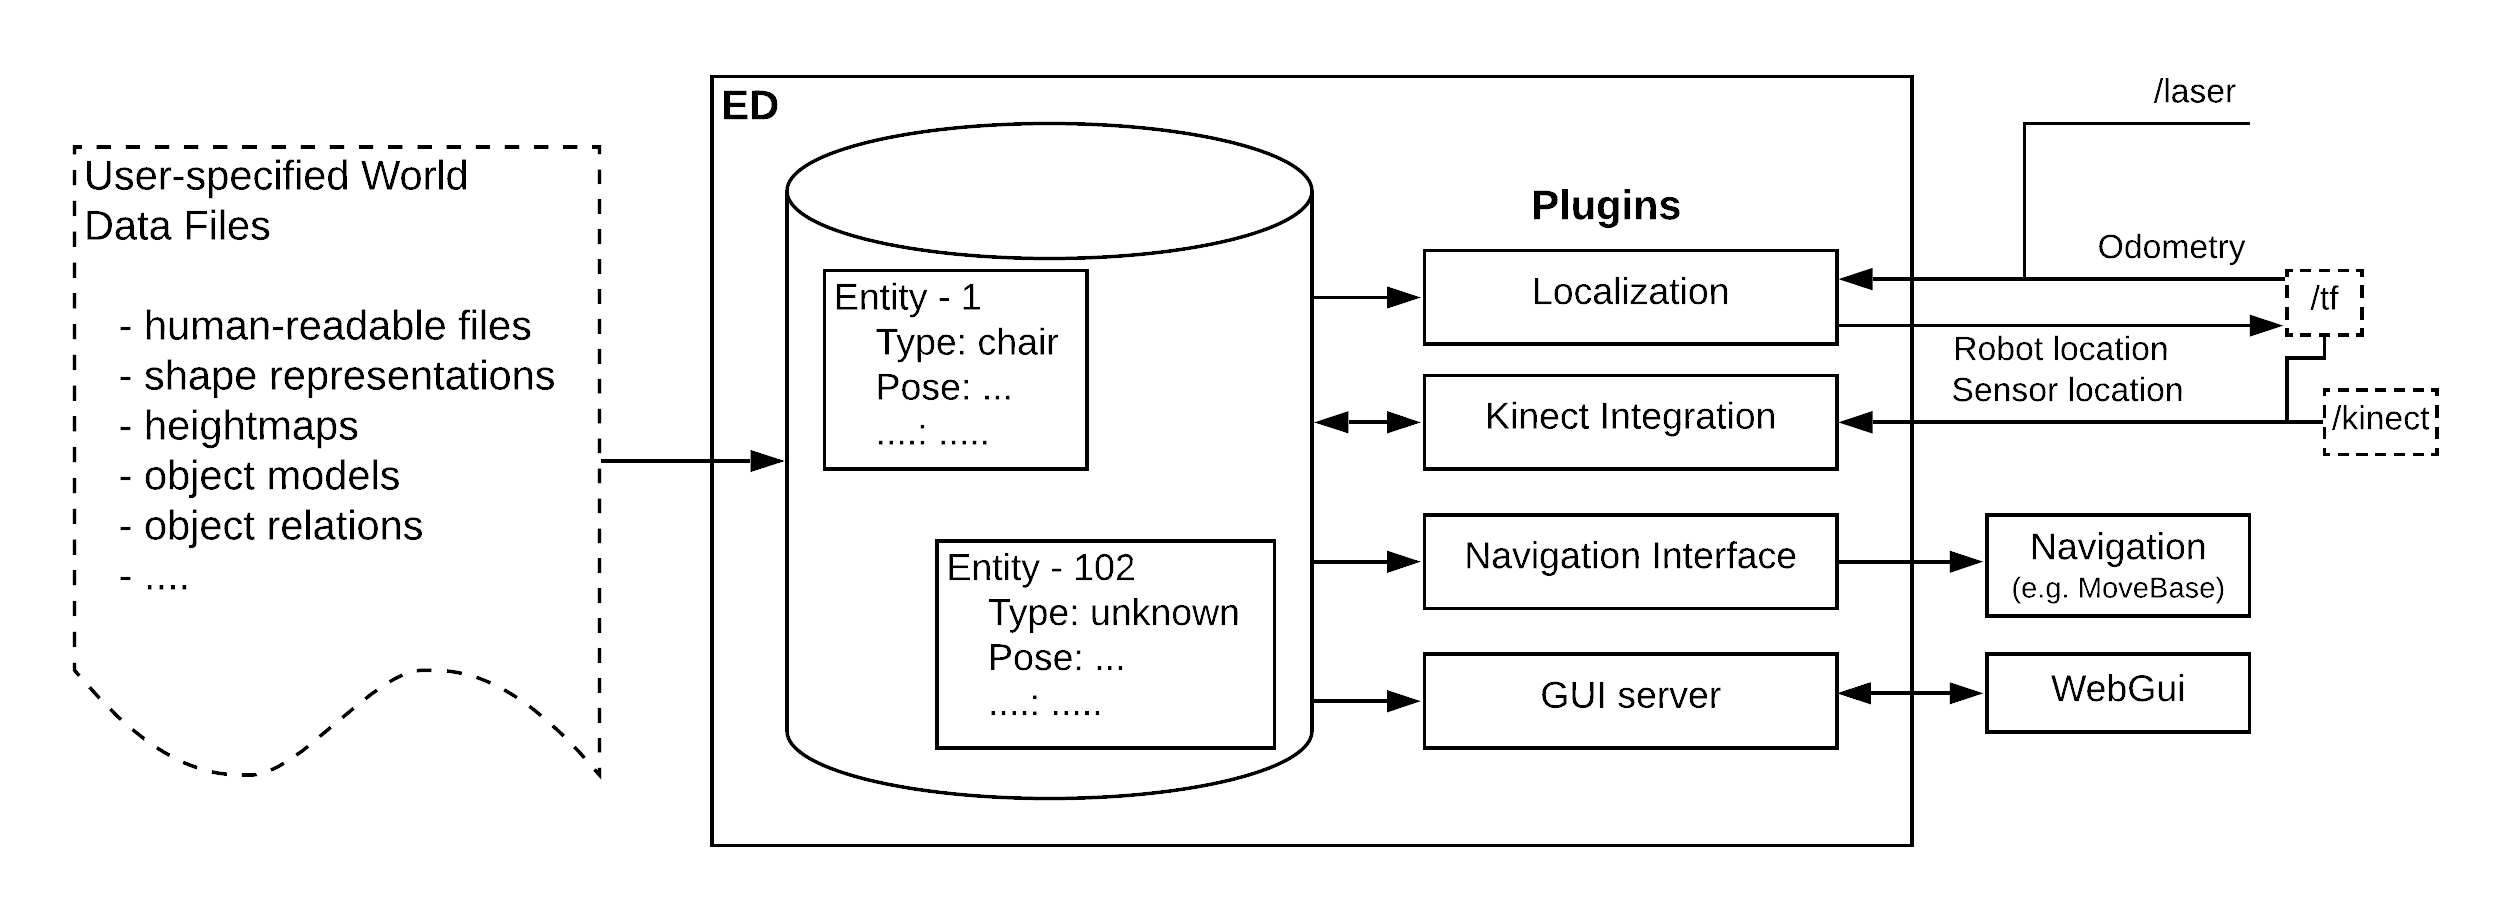
\includegraphics[width = 0.9\linewidth]{Figures/ed_overview}
    %\vspace{-1em}
	\caption{schematic overview of TUe Environment Descriptor.}
	\label{fig:ed}
    %\vspace{-0.5cm}
\end{figure}
ED is one re-usable environment description that can be used for a multitude of needed functionalities. Instead of having different environment representations for localization \acrfull{amcl}, navigation (MoveBase), manipulation (MoveIt!), interaction, etc.. An improvement in this single, central world model will reflect in the performances of the separate robot capabilities. It omits updating and synchronization of multiple world models. At the moment different ED plugins exist that enable robots to localize themselves, update positions of known objects based on recent sensor data, segment and store newly encountered objects and visualize all this through a web-based \acrshort{gui}, illustrated in Figure \ref{fig:gui_actions}.
\begin{figure}[h]
\centering
    %\vspace{-0.3cm}
	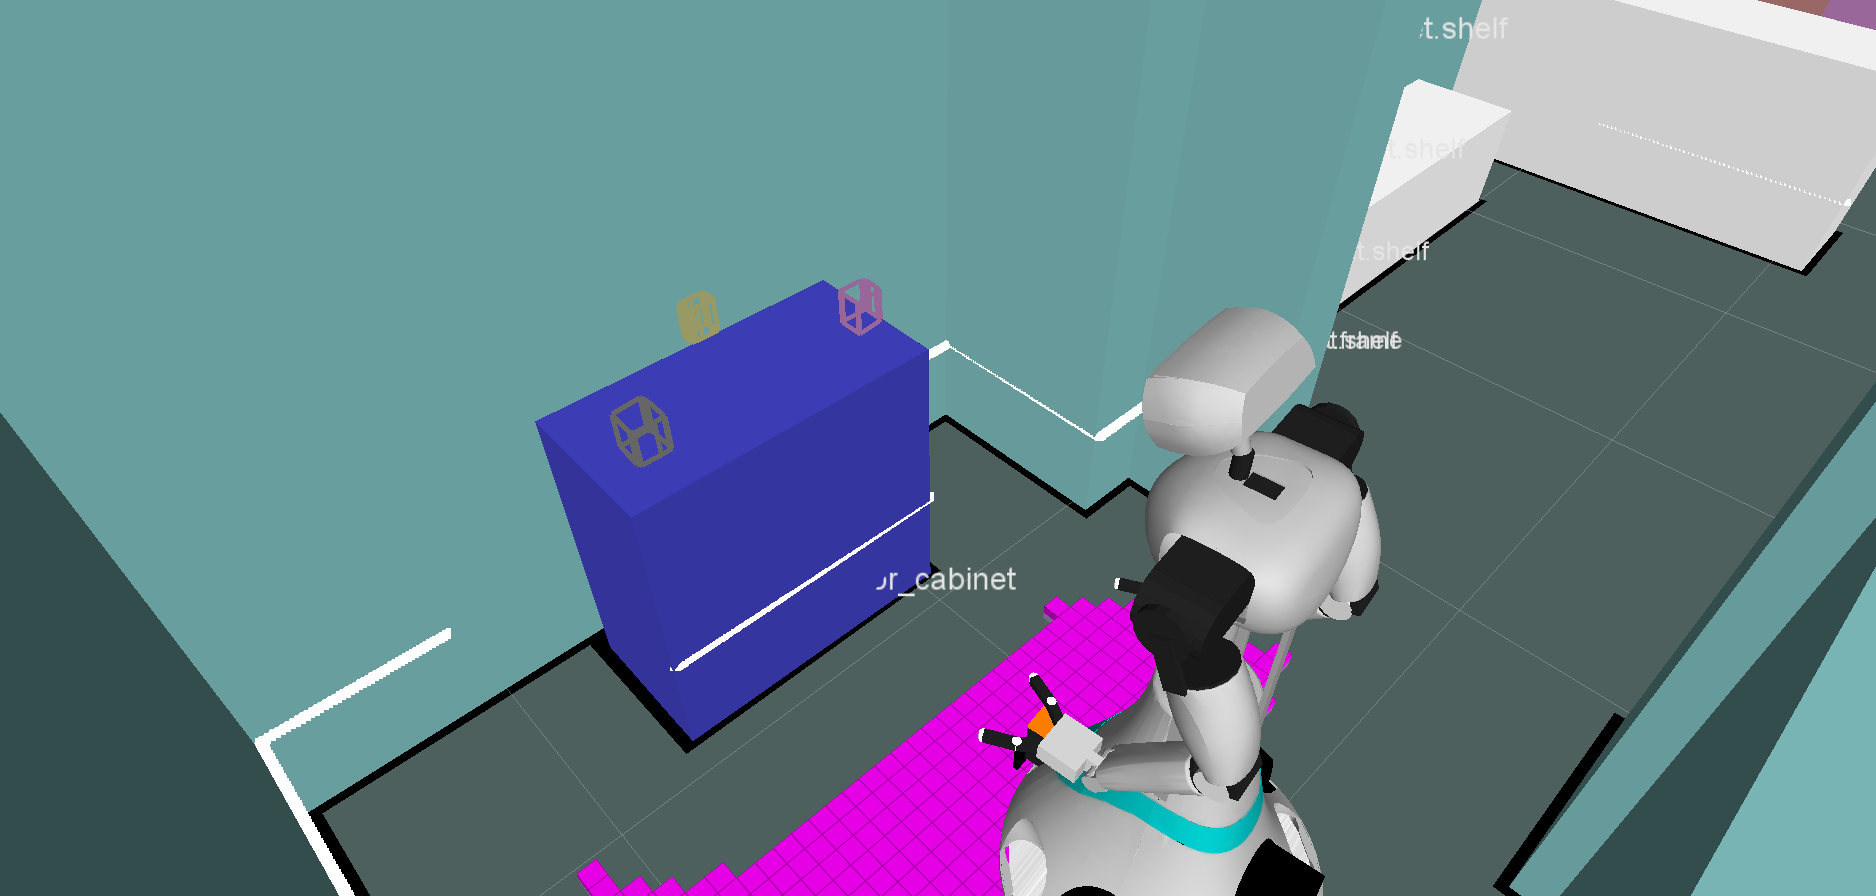
\includegraphics[width = 0.8\linewidth]{Figures/ed_segmentation}
    %\vspace{-0.5em}
	\caption{A view of the world model created with ED. The figure show the occupation grid as well as (unknown) objects recognized on top of the cabinet.}
	\label{fig:ed_segmentation}
    %\vspace{-0.5cm}
\end{figure}



\subsection{Localization, Navigation and Exploration}
The \emph{ed\_localization}\footnote{\url{https://github.com/tue-robotics/ed_localization}} plugin implements \acrshort{amcl} based on a 2D render of the central world model.
\\
With use of the \emph{ed\_navigation} plugin\footnote{\url{https://github.com/tue-robotics/ed_navigation}}, an occupancy grid is derived from the world model and published.
\\
With the use of the \emph{cb\_base\_navigation} package\footnote{\url{https://github.com/tue-robotics/cb_base_navigation}} the robots are able to deal with end goal constraints. The \emph{ed\_navigation} plugin allows to construct such a constraint w.r.t. a world model entity in \acrshort{ed}. This enables the robot to navigate not only to areas or entities in the scene, but to waypoints as well. Figure \ref{fig:ed_segmentation} also shows the navigation to an area.
% as illustrated by Figure \ref{fig:ed_navigation_constraints}.
Modified versions of the local and global ROS planners available within \emph{move\_base} are used.


\subsection{Object detection}
\subsubsection{Detection \& Segmentation}
ED enables integrating sensors through the use of the plugins present in the \textit{ed\_sensor\_integration} package. Two different plugins exist:
1. The \emph{laser\_plugin}: Enables tracking of 2D laser clusters. This plugin can be used to track dynamic obstacles such as humans.
2. The \emph{kinect\_plugin}: Enables world model updates with use of data from a RGBD camera. This plugin exposes several ROS services that realize different functionalities:
\begin{enumerate}[label=(\alph*)]
\item Segment: A service that segments sensor data that is not associated with other world model entities. Segmentation areas can be specified per entity in the scene. This allows to segment object `on-top-of’ or ‘in’ a cabinet. All points outside the segmented area are ignore for segmentation.
\item FitModel: A service that fits the specified model in the sensor data of a RGBD camara. This allows updating semi-static obstacles such as tables and chairs.
\end{enumerate}


The \emph{ed\_sensor\_integration} plugins enable updating and creating entities. However, new entities are classified as unknown entities. Classification is done in \emph{ed\_perception} plugin\footnote{\url{https://github.com/tue-robotics/ed_perception}} package. 

\subsection{Object grasping, moving and placing}
The system architecture developed for object manipulation is focused on grasping. In the implementation, its input is a specific target entity in \acrshort{ed}, selected by a Python executive and the output is the grasp motion joint trajectory.
Figure \ref{fig:grasping_pipeline} shows the grasping pipeline.
\begin{figure}[H]
    \centering
    %\vspace{-0.3cm}
	\includegraphics[width = 1\linewidth]{Figures/grasping_pipeline}
    %\vspace{-1em}
	\caption{Custom grasping pipeline base on \acrshort{ed}, MoveIt and a separate grasp point determination and approach vector node.}
	\label{fig:grasping_pipeline}
    %\vspace{-0.5cm}
\end{figure}
\noindent MoveIt! is used to produce joint trajectories over time, given the current configuration, robot model, \acrshort{ed} world model (for collision avoidance) and the final configuration.
%\acrshort{ed} provides collision meshes to MoveIt! so it can plan paths that avoid obstacles.
%Finally, the trajectories are sent to the reference interpolator which sends the trajectories either to the controllers or the simulated robot.
%The grasping pipeline is extended with an empty spot designator and grasping pose determination. The empty spot designator searches in an area, like `on-top-of'of the dinner table, for an empty spot to place an object by using the occupied area by other objects in this area.
The grasp pose determination uses the information about the position and shape of the object in \acrshort{ed} to determine the best grasping pose.
The grasping pose is a vector relative to the robot.
%An example of the determined grasping pose is shown in Figure \ref{fig:grasping_pose_determination}.
Placing an object is approached in a similar manner to grasping, except for that when placing an object, \acrshort{ed} is queried to find an empty placement pose.

%
%\begin{figure}[H]
%   \centering
%   %\vspace{-0.3cm}
%   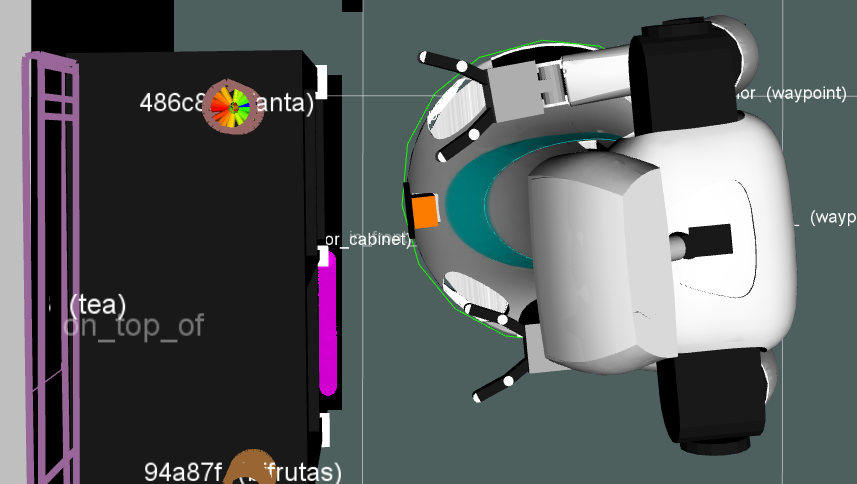
\includegraphics[width = 0.8\linewidth]{Figures/grasp_point_determination}
%    %\vspace{-1em}
%	\caption{Grasping pose determination result for a cylindric object with %TU/e built robot AMIGO. It is unpreferred to grasp the object from behind.}
%	\label{fig:grasping_pose_determination}
%    %\vspace{-0.5cm}
%\end{figure}


\section{Image Recognition}
The \emph{image\_recognition} packages apply state of the art image classification techniques based on \acrfull{cnn}.
%\begin{figure}[H]
%    \centering
%    %\vspace{-0.3cm}
%	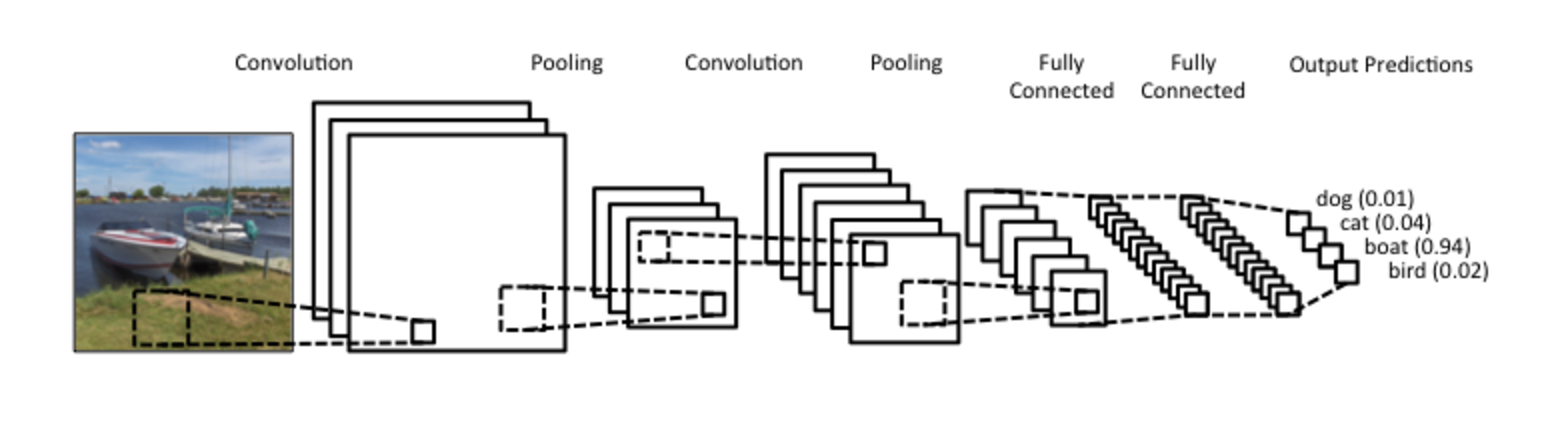
\includegraphics[width = 1\linewidth]{Figures/cnn}
%    %\vspace{-1em}
%    \caption{Illustration of \acrfull{cnn} used in our object recognition nodes with use of Tensorflow.}
%	\label{fig:cnn}
%    %\vspace{-0.5cm}
%\end{figure}

\subsection{Object recognition using Deep Learning}
Object recognition is done using Tensorflow\texttrademark\hspace{0em} by retraining the top-layer of a Inception V3 neural network. 
The top layers are retrained on a custom dataset using a soft-max top-layer that maps the image representation on a specified set of labels.
\\
In order to create a new training set for specific objects the \emph{image\_recognition} packages contain several tools for annotating objects. 
Tools for retraining neural networks are also included.

\subsection{Face recognition}
Face detection and recognition is done using OpenFace\footnote{\url{https://cmusatyalab.github.io/openface/}} based on Torch. 
%OpenFace is an existing state-of-the-art face recognition library. We implemented a ROS node that enables the use of these advanced technologies within the ROS network.
\subsection{ROS packages}
Our image recognition ROS packages can be found on GitHub\footnote{\url{https://github.com/tue-robotics/image_recognition}} together with tutorials and documentation. 
Recently, they have also been added to the ROS Kinetic package list and can be installed as Debian packages: \emph{ros-kinetic-image-recognition} 

\section{People Recognition}
\label{sec:pers_recog}
As our robots need to operate and interact with people in a dynamic environment, our robots’ people detection skills have been upgraded to a generalized system capable of recognizing people in 3D.
In the people recognition stack, an RGB-D camera is used as the sensor to capture the scene information. A recognition sequence is completed in four steps. First, people are detected in the scene using OpenPose and if their faces are recognized, using OpenFace, as one of the learned faces in the robot's database, they are labeled using their known name.
The detections from OpenPose are associated with the recognitions from OpenFace by maximizing the IoUs of the face ROIs. Then, for each of the recognized people, additional properties such as age, gender and the shirt color are identified. Furthermore, the pose keypoints of these recognitions are coupled with the depth information of the scene to re-project the recognized people to 3D as skeletons. Finally, information about the posture of each 3D skeleton is calculated using geometrical heuristics.
This allows for the addition of properties such as “pointing pose” and additional flags such as `is\_waving', `is\_sitting', etc.
%The current design of our people recognition stack is loosely coupled. In the future, the design will be completely decoupled into the individual components, as most challenges do not require all the information generated by this system.
%
%\begin{figure}[H]
%	\centering
%    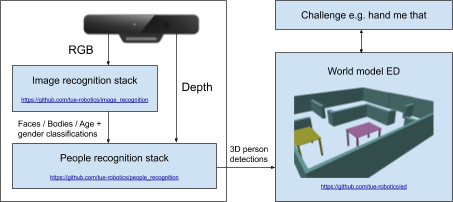
\includegraphics[width=0.7\linewidth]{pointing_pose}
%	\caption{The person detection pipeline}
%	\label{fig:people_recognition}
%\end{figure}
\subsection{Pointing detection}
In the previous section, our approach to people recognition is explained. This recognition includes information about the posture of each 3D skeleton. Once the people information is inserted into the world model, additional properties can be added to the persons that take also other entities in the world model into account, e.g. `is\_pointing\_at\_entity'. This information is used by the toplevel state machines to implement challenges.
However an additional check based on spatial queries is inserted to ensure that the correct operator is found. By using such a query it is possible to filter out people based on their location. Finally, to determine at which entity the operator is pointing, ray-tracing is implemented. Figure \ref{fig:ray_trace} shows an example of the ray-tracing.

\begin{figure}[H]
	\centering
    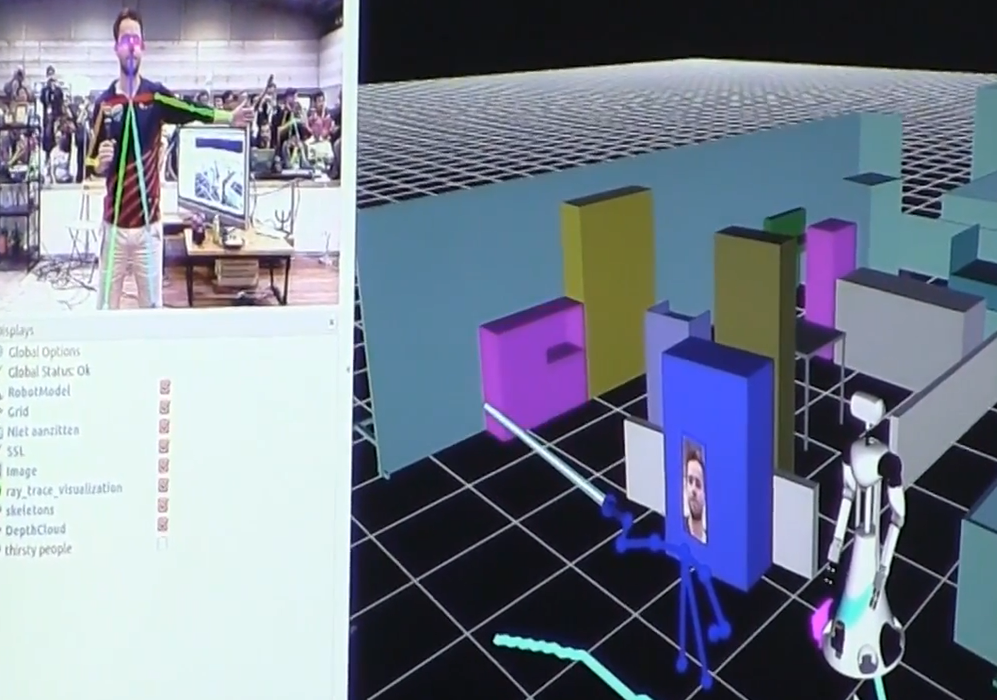
\includegraphics[width=0.8\linewidth]{ed_ray_trace2}
	\caption{Ray-tracing based on pose detection with AMIGO.}
	\label{fig:ray_trace}
\end{figure}

%\section{Pose detection}
%Pose detection is done with OpenPose\footnote{\url{https://github.com/CMU-Perceptual-Computing-Lab/openpose}}.
OpenPose is a real-time multi-person keypoint detection library for body, face, and hands.
It's used for example in the restaurant challenge to detect waving persons.
In the finals we used it to detect when an operator points to objects in the living room.
For that we ray-traced the vector of the arm in our world model and extracted the first object that the ray intersects.
This enables the robot to understand commands like: ``Give me \emph{that} object''.
See figure~\ref{fig:pose_detection} for an example of the output of the algorithm.

\begin{figure}[H]
	\centering
	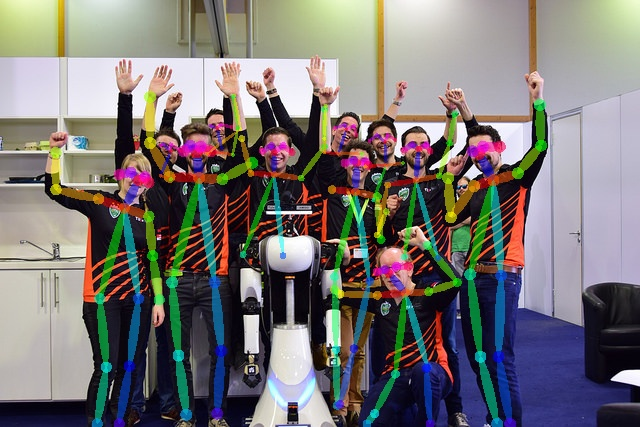
\includegraphics[width=0.66\linewidth]{openpose}
	\caption{Pose detection}
	\label{fig:pose_detection}
\end{figure} 

%\section{Sound source localization}
%To perform proper speech recognition, the direction of the sound is important to capture the sound source properly. We localize the sound source by determining the direction of arrival (DOA) with use of the microphone array board with 8 microphones\footnote{\url{https://creator.matrix.one}} of the Matrix Creator.
%depicted in Figure \ref{fig:matrix_one}.
%\begin{figure}[h]
%    \centering
%    %\vspace{-0.3cm}
%	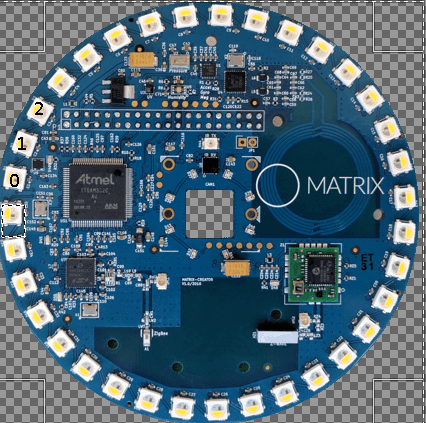
\includegraphics[width = 0.5\linewidth]{Figures/ssl_Matrix_creator.png}
%    %\vspace{-1em}
%	\caption{Matrix One Creator board.}
%	\label{fig:matrix_one}
%    %\vspace{-0.5cm}
%\end{figure}
The detection is done by first calculating the time cross correlation between four pairs of opposing microphones. Second, the microphone pair with the lowest phase shift w.r.t. the opposing microphone is selected as being perpendicular to the source. Finally, the direction of the source can be determined by combining this information with the energy level\footnote{\url{https://github.com/tue-robotics/matrix-creator-hal}} of the microphones. Our software for the DOA detection is available on GitHub, as well as a ROS package\footnote{\url{https://github.com/tue-robotics/matrix_creator_ros}} that exposes the DOA detections via a geometry\_msgs/PoseStamped topic interface. 

%\subsection{Reasoning}	
%The reasoning layer of the AMIGO ROS based software consists of a set of finite state machines (robot\_smach\_states\footnote{\url{https://github.com/tue-robotics/robot_smach_states}}) that build upon the robot’s skill layer (robot\_skills\footnote{\url{https://github.com/tue-robotics/robot_skills}}). These state machines are useful if you want the robot to execute some complex plan, where all possible states and state transitions can be described explicitly. The implementation is done with use of the open-source SMACH package. %SMACH is a task-level architecture for rapidly creating complex robot behaviours. 

%\newpage
\section{Human-Robot Interface}
The acceptance of a robot is largely determined by the interaction with it. Hence, we try to have multiple ways of interacting with the robot in an intuitive manner. The two highlighted in this paper are our WebGUI, subsection \ref{ssec:webgui}, and Telegram\texttrademark\hspace{0em} interface, subsection \ref{ssec:telegram}, which uses our \emph{conversation\_engine}, subsection \ref{ssec:conversation}.

\subsection{Web GUI}
\label{ssec:webgui}
In order to interact with the robot, apart from speech, we have designed a web-based \gls{gui}. This interface uses HTML5\footnote{\url{https://github.com/tue-robotics/tue_mobile_ui}} with the Robot API written in Javascript and we host it on the robot itself.
%This allows multiple users on different platforms (\eg\ Android, iOS) to access functionalities of the robot. The interface is implemented in JavaScript with AngularJS and it offers a graphical interface to the Robot API\footnote{\url{https://github.com/tue-robotics/robot-api}} which exposes all the functionality of the robot.
%\begin{figure}[h]
%    \centering
%	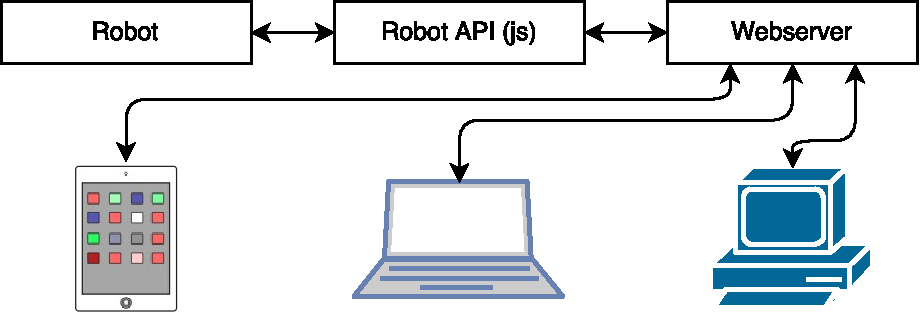
\includegraphics[width=0.9\linewidth]{Figures/webgui_architecture}
%    %\vspace{-0.5em}
%	\caption{
%		Overview of the WebGUI architecture.
%		A webserver that is hosting the \protect\gls{gui} connects this %Robot API to a graphical interface that is offered to multiple clients on %different platforms.}
%	\label{fig:webgui_architecture}
%\end{figure}
%Figure~\ref{fig:gui_actions} gives an example of various user interactions that are possible with the \gls{gui} and the different commands that can be given to the robot while interacting with the virtual scene.

\begin{figure}[H]
	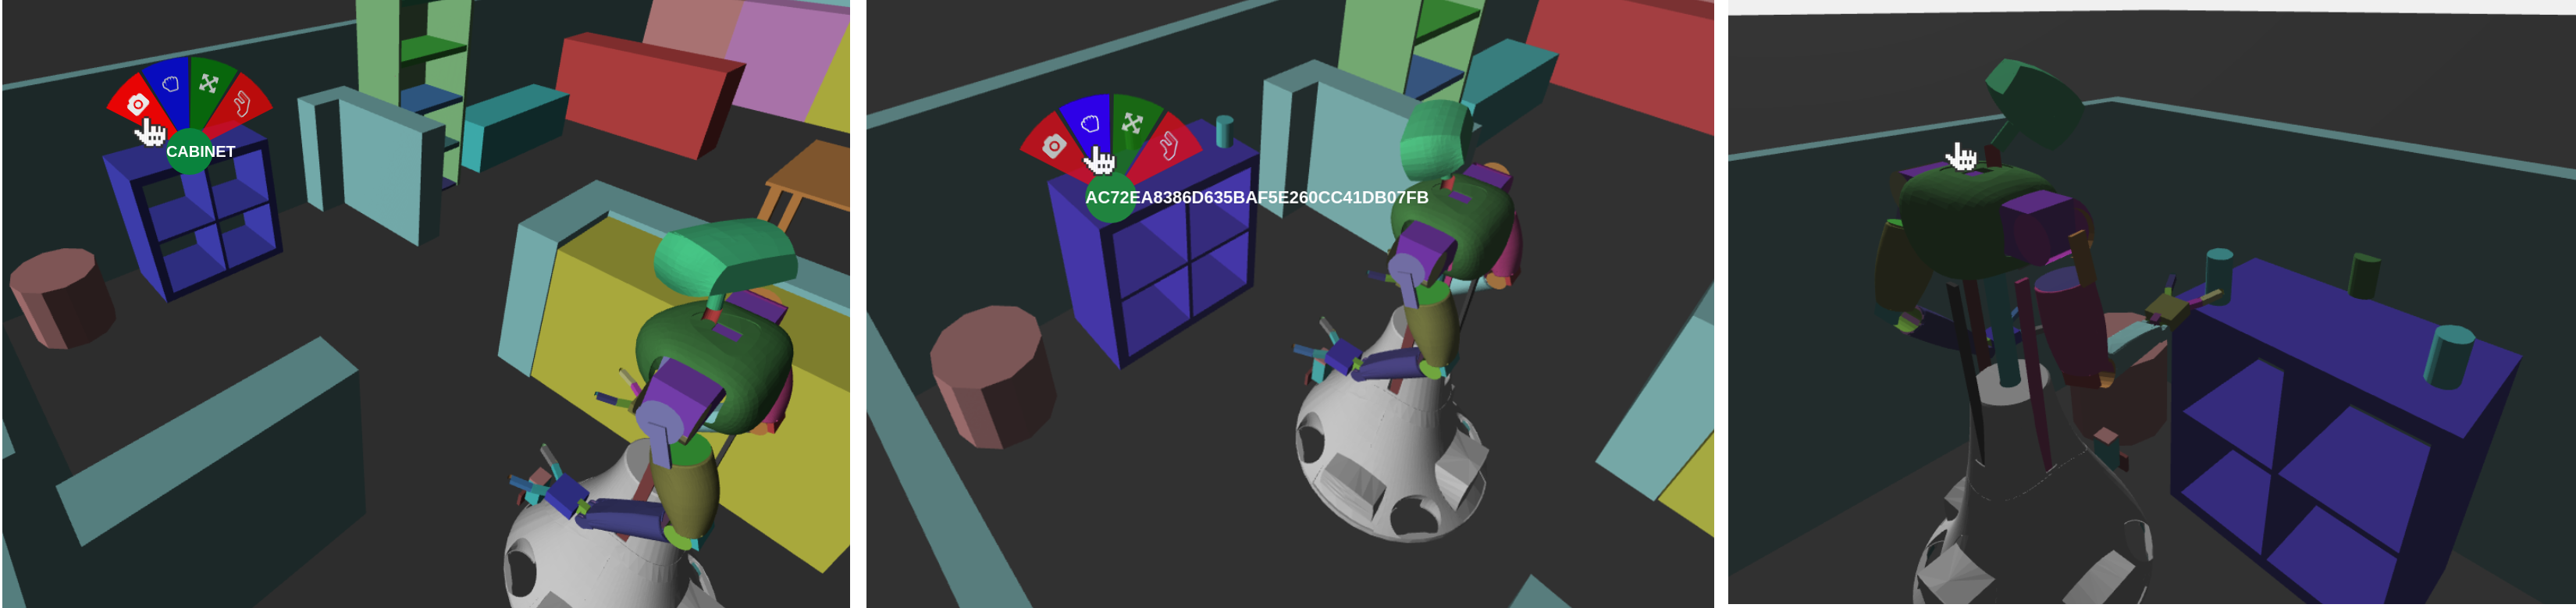
\includegraphics[width=\linewidth]{Figures/gui_actions}
	\caption{
		Illustration of the 3D scene of the WebGUI with AMIGO.
		User can long-press objects to open a menu from which actions on the object can be triggered
%		Users can interact with use of the menu that appears when long pressing an object in the scene.
%		On the left figure, the user commands the robot to inspect the selected object, which is the `cabinet'.
%		When the robot has inspected the `cabinet', it has found entities on top of it.
%		In the middle figure a grasp command is given to the robot to pick up an object from the cabinet.
%		The last figure show the robot executing that action.
		}
	\label{fig:gui_actions}

\end{figure}
%Figure \ref{fig:webgui_architecture} gives an overview of the connections between these components and 
\noindent Figure \ref{fig:gui_actions} represents an instance of the various interactions that are possible with the Robot API.

\subsection{Telegram\texttrademark\hspace{0em}}
The telegram interface\footnote{\url{https://github.com/tue-robotics/telegram_ros}}to our robots is a ROS wrapper around the \textit{python-telegram-bot} library. The software exposes four topics. It accepts both text and images to and from the robot. The interface allows only one master of the robot at a time. To gain ownership over the robot, you need to sent \textit{/start}.

The interface itself doesn't contain any reasoning. This is all done by the conversation engine.

\subsubsection{Conversation Engine}\

The conversation engine\footnote{\url{https://github.com/tue-robotics/conversation_engine}} bridges the gap between text input and an action planner (called action\_server). Text can be received from either Speech-to-Text or from a chat interface, like Telegram\texttrademark\hspace{0em}.
The text is parsed according to a (Feature) Context Free Grammar, resulting in an action description in the form of a nested mapping. In the action description, (sub)actions and their parameters are filled it. This may include references such as 'it'.

Based on the action description, the action server tries to devise a sequence of actions and parameterize those with concrete object IDs. It may be that more information is needed (e.g. "Place a coke on the dinner table"). The action then fails for this reason and then the conversation engine must interact with the user to obtain the missing information (e.g. "Where should I pick that up?").

When the user supplies more information, the input is parsed and the current action description is extended and retried. To parse the additional information to fill in gaps of missing info, the conversation engine must know what field of missing information (e.g. 'source-location' of a 'grab' action) must be parsed according to what rules. The conversation engine is therefore parameterized with a mapping that links fields containing e.g. 'location' to a rule in the grammar called 'LOCATION'.

Lastly, it keeps the user 'informed' while actions are being performed by reporting on the current subtask.

\subsubsection{Custom Keyboard, Telegram HMI}\

\label{ssec:keyboard}
\noindent To reduce the operator error, we only present the user with a limited number of buttons in the Telegram app using its \emph{custom\_keyboards} feature. %This feature is especially useful if there are only a few options, such as when selecting from a predetermined selection of drinks.
This feature has been employed to compose commands word-for-word. After the user has  entered a partial command, for example “Bring me the ...” they are presented with only those words that might follow that text according to the grammar, eg. “apple”, “orange” etc. This process iterates until a full command has been composed.


\subsection{Head Display}
\label{ssec:display}
For most people, especially people who do not deal with robots in their day-to-day life, interaction with robots is not as easy as one would like it to be.
% It is often difficult to hear what the robot is saying and it is not always intuitive for people to know when to talk to the robot. 
To remedy this, the head display of HERO is used. On this display that is integrated in the Toyota HSRs' 'head', a lot of useful information can be displayed. Through the \emph{hero\_ display}\footnote{\url{https://github.com/tue-robotics/hero-display}} a few different functionalities are integrated. As per default, our Tech United @Home logo with a dynamic background is shown on the screen, as depicted in Figure \ref{fig:hero_display}. When the robot is speaking the spoken text is displayed, when the robot is listening a spinner along with an image of a microphone is shown and it is possible to display images.
\begin{figure}[H]
    \centering
	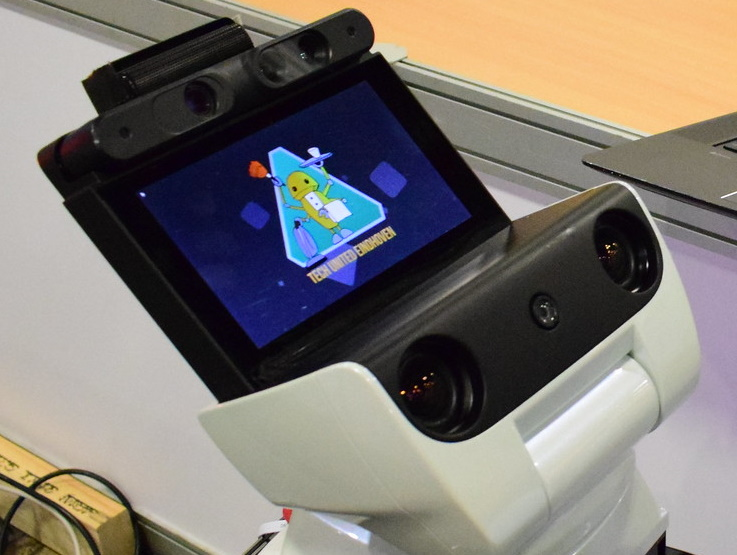
\includegraphics[width=0.45\linewidth]{hero_display_live}
    %\vspace{-0.5em}
	\caption{
		The default status of HERO's head display.}
	\label{fig:hero_display}
\end{figure}


\section{Re-usability of the system for other research groups}
Tech United takes great pride in creating and maintaining open-source software and hardware to accelerate innovation. Tech United initiated the Robotic Open Platform website\footnote{\url{http://roboticopenplatform.org/}}, to share hardware designs. All packages are equipped with documentation and tutorials. Tech United and its scientific staff have the capacity to co-develop (+10 people), maintain and assist with questions

\section{Community Outreach and Media}
The Tech United team carries out many promotional activities for children to promote technology and innovation. These activities are performed by separate teams of student assistants. Tech United often visits primary and secondary schools, public events, trade fairs and has regular TV appearances. In 2015 and 2016 combined, 100+ demos were given and an estimated 50k people were reached through live interaction.
Tech United also has a very active website\footnote{\url{http://www.techunited.nl}}, and interacts on many social media like: Facebook\footnote{\url{https://www.facebook.com/techunited}}, YouTube\footnote{\url{https://www.youtube.com/user/TechUnited}}, Twitter\footnote{\url{https://www.twitter.com/TechUnited}} and Flickr\footnote{\url{https://www.flickr.com/photos/techunited/}}. Our robotics videos are often shared on the IEEE video Friday website. 


%%%%%%%%%%%%%%%%%%%%%%%%%%%%%%%%%%%%%%%%%%%%%%%%%%%%%%%%%%%%%%%%%%%%%%%%%%%%%%%%%%%%%
%%
%% Bibliography\usepackage{graphicx}
%%
%%%%%%%%%%%%%%%%%%%%%%%%%%%%%%%%%%%%%%%%%%%%%%%%%%%%%%%%%%%%%%%%%%%%%%%%%%%%%%%%%%%%%

%\section*{Bibliography}
\bibliographystyle{unsrt}
\bibliography{refs}

%%%%%%%%%%%%%%%%%%%%%%%%%%%%%%%%%%%%%%%%%%%%%%%%%%%%%%%%%%%%%%%%%%%%%%%%%%%%%%%%%%%%%
%%
%% Robot Specifications
%%
%%%%%%%%%%%%%%%%%%%%%%%%%%%%%%%%%%%%%%%%%%%%%%%%%%%%%%%%%%%%%%%%%%%%%%%%%%%%%%%%%%%%%
%
%\robospecs
\newpage
%\section{Robot Description}
\section*{HSR's Software and External Devices}
% In this section briefly describe the software and hardware of the robot

\setlength\intextsep{0pt}
\begin{wrapfigure}[5]{r}{0.3\textwidth}
	\centering
	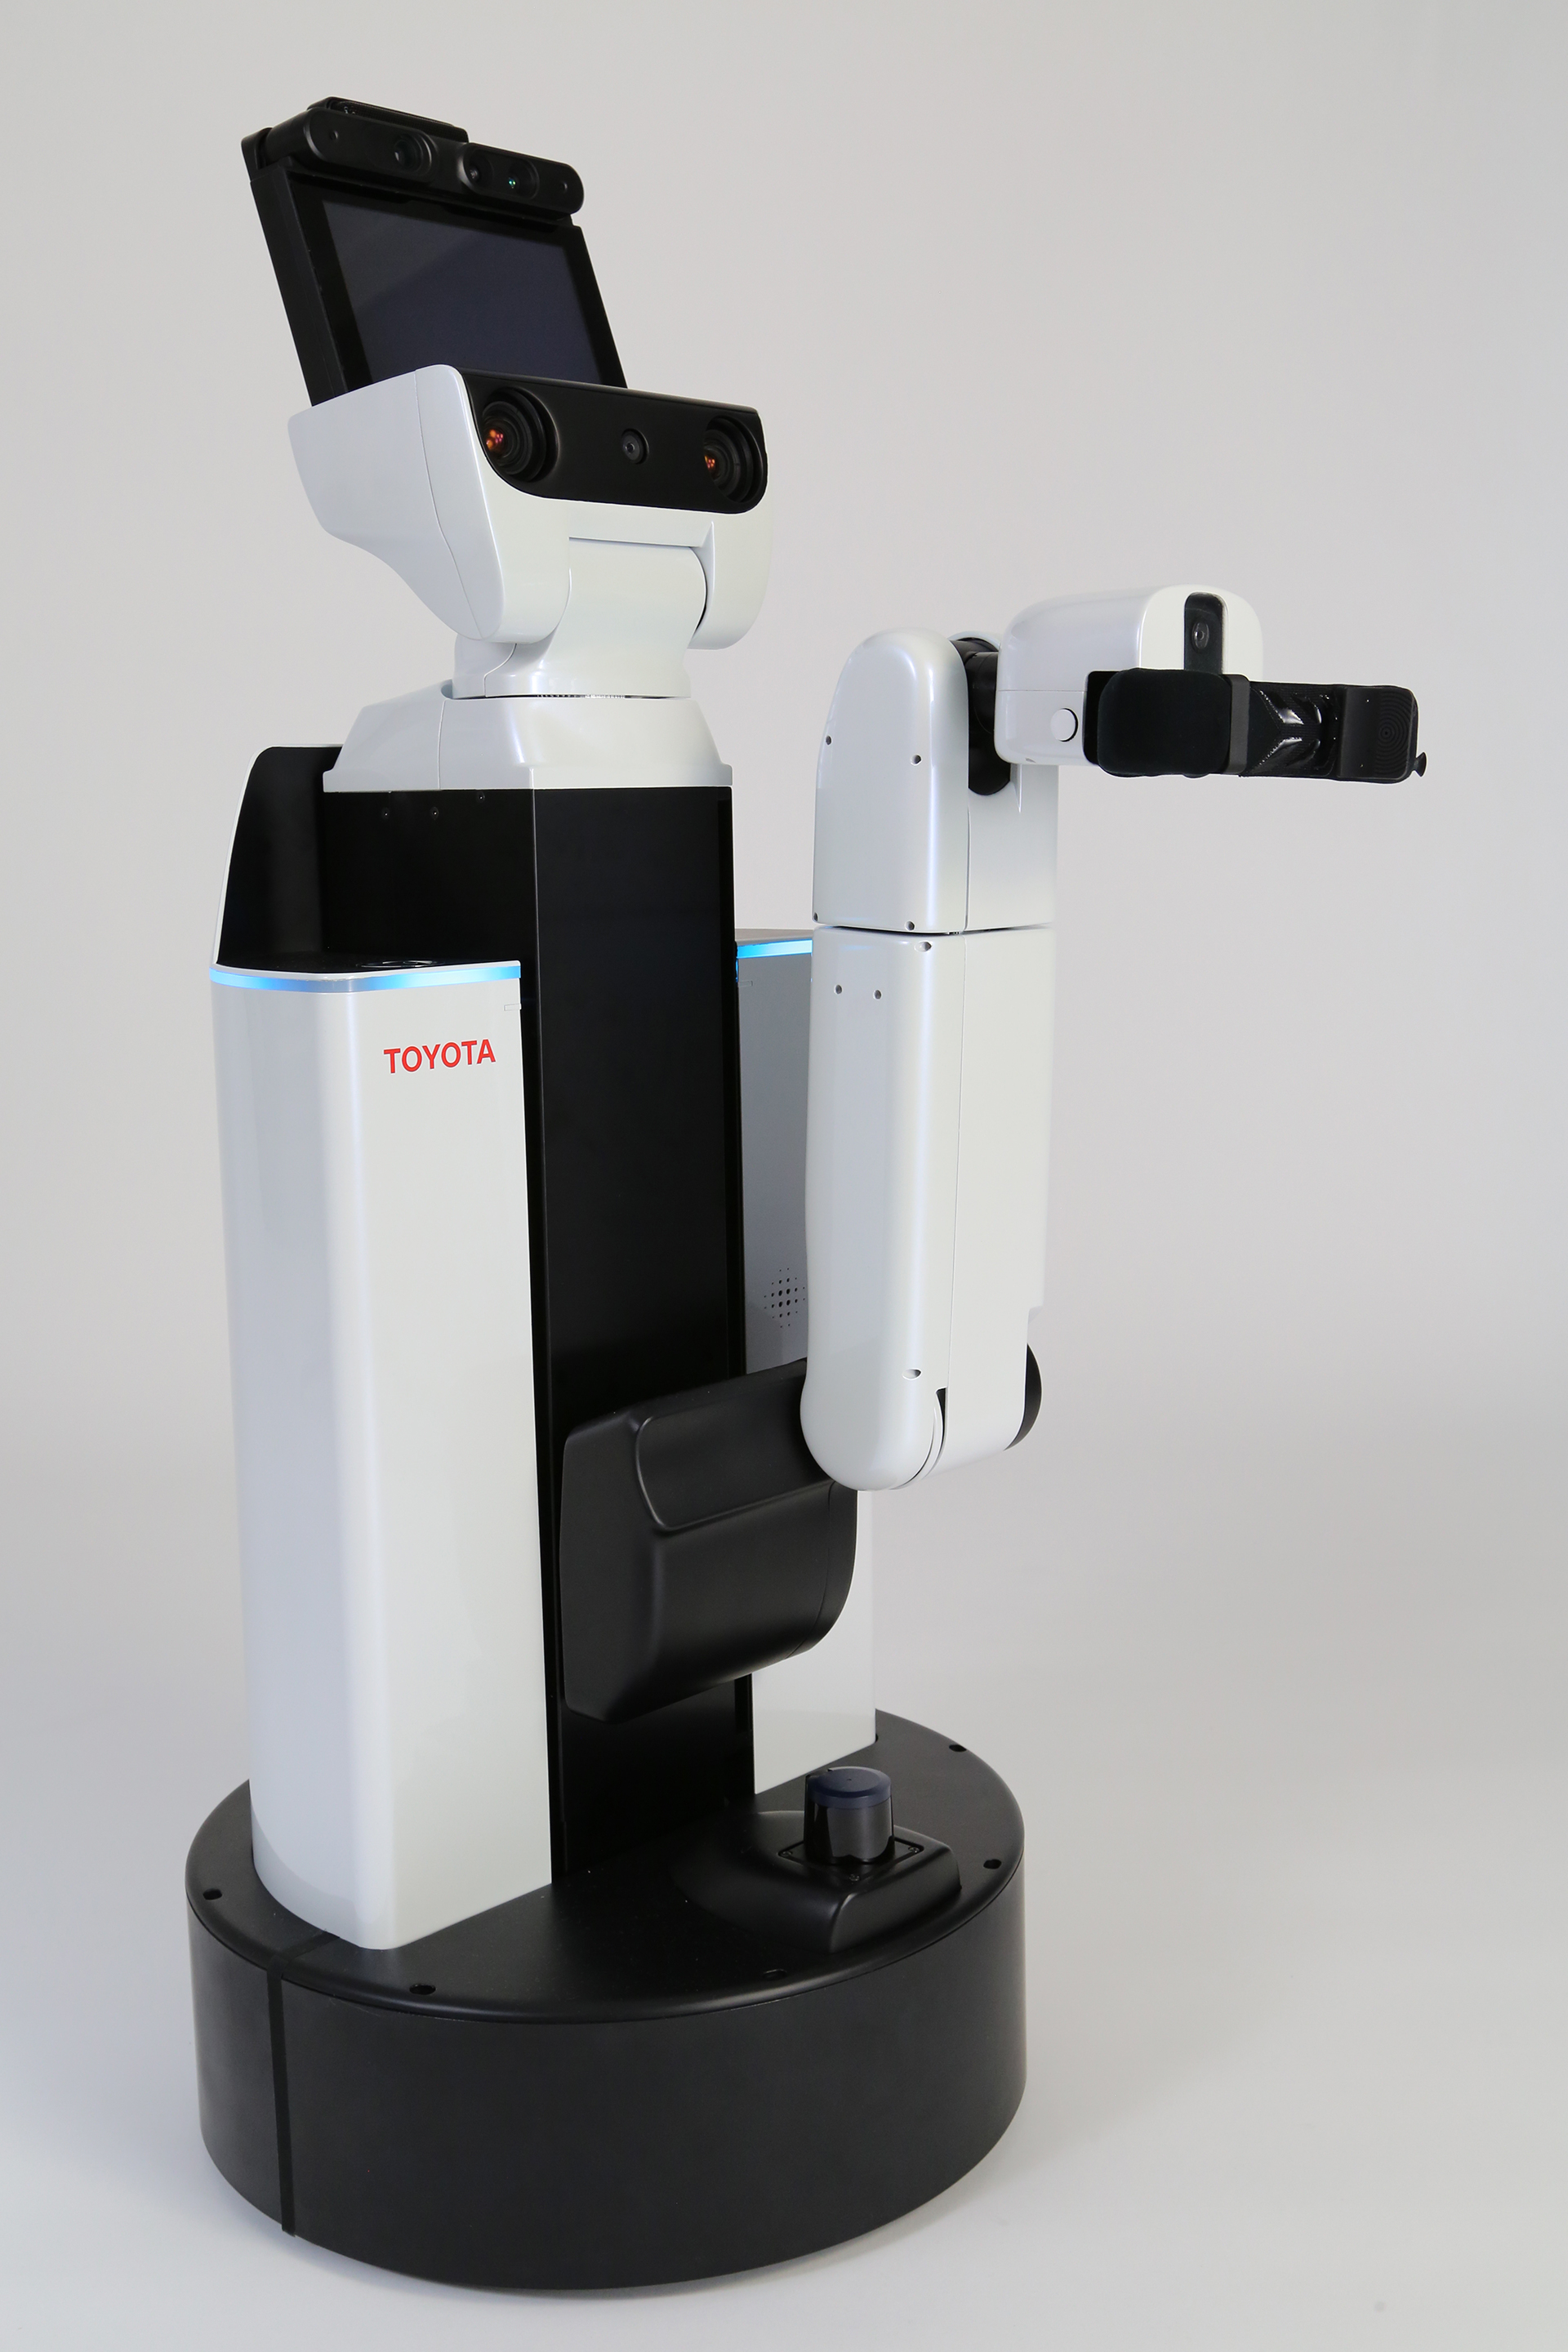
\includegraphics[width=0.3\textwidth]{Toyota_HSR}
	\caption{The Toyota HSR Robot, HERO}
	\label{fig:hsr}
\end{wrapfigure}

We use a standard \textit{Toyota} HSR robot unit. To differentiate our unit, we named it HERO. We wanted to link the name to our AMIGO and SERGIO domestic service robots.

\section*{HERO's Software Description}
% Please describe in this section the software you are using to control your robot. Consider the following example:

An overview of the software used by the Tech United Eindhoven @Home robots can be found in Table~\ref{tab:softwarespec}.
All our software is developed open-source at GitHub\footnote{\url{https://github.com/tue-robotics}}.
\\\newline
Currently, we have some \textit{image\_recognition} packages released into the current ROS Kinetic distribution and can be installed with use of \textit{apt}.

\begin{table}[H]
    \begin{center}
    \caption{Software overview of the robots.}
    \label{tab:softwarespec}
    %\vspace{-0.1cm}
    \renewcommand{\arraystretch}{1.0}
    \setlength{\tabcolsep}{5pt}
        \begin{tabular}{p{0.3\textwidth} p{0.7\textwidth}}
            \toprule
            Operating system & Ubuntu 16.04 LTS Server\\

            Middleware & ROS Kinetic~\cite{Quigley2009}\\

            Low-level control software & Orocos Real-Time Toolkit~\cite{Bruyninckx2001}\newline
            \url{https://github.com/tue-robotics/rtt_control_components}
            \\

            Simulation & Custom kinematics + sensor simulator \newline
            \url{https://github.com/tue-robotics/fast_simulator}
            \\

            World model & \acrfull{ed}, custom \newline
            \url{https://github.com/tue-robotics/ed}\\

            Localization & Monte Carlo~\cite{Fox2003} using \gls{ed}, custom \newline \url{https://github.com/tue-robotics/ed\_localization}\\

            SLAM & Gmapping package \newline \url{http://wiki.ros.org/gmapping}\\

            Navigation & CB Base navigation
            \newline
            \url{https://github.com/tue-robotics/cb_base_navigation}
            \newline
            Global: custom A* planner\newline Local: modified ROS DWA~\cite{Fox1997}\\

            Arm navigation & Custom implementation using MoveIt and Orocos KDL\newline
            \url{https://github.com/tue-robotics/tue_manipulation}
            \\

            Object recognition & Tensorflow ROS \newline
			\url{https://github.com/tue-robotics/image\_recognition/tree/master/tensorflow\_ros}\\

            People detection & Custom implementation using contour matching \newline
            \url{https://github.com/tue-robotics/ed_perception}
            \\
            Face detection \& recognition & Openface ROS \newline \url{https://github.com/tue-robotics/image\_recognition/tree/master/openface\_ros} \\

            Speech recognition & Julius Speech Recognition \newline
            \url{https://github.com/julius-speech/julius}\\
            Speech synthesis & Toyota\texttrademark \hspace{0em} Text-to-Speech\\
            Task executors & SMACH \newline
            \url{https://github.com/tue-robotics/tue_robocup}\\
            \bottomrule
        \end{tabular}
    \end{center}
\end{table}

This our current software implementation on our robots AMIGO and SERGIO, which participate in the open league. Because of the pending delivery of the Toyota HSR and related documentation, we are not able to provide the specific software implementation. As described in our selection qualification paper, our goal is to use the same software as possible on all our robots, including the Toyota HSR.

\section*{External Devices}
% Please describe in this section the external devices used by your robot. Consider the following example:

\textit{HERO relies on the following external hardware:}

\begin{itemize}
	\item Mother-ship
	\item Data Cluster
	\item $3 \times$ Ultra-Power laptops.
\end{itemize}

\section*{Cloud Services}
% Please describe in this section the Cloud Services and online software used by your robot. Consider the following example:

\textit{HERO connects the following cloud services:}
\begin{itemize}
	\item Localization and mapping: Geolocalization system.
	\item Navigation: Navigator
	\item Speech recognition: All-purpose recognizer.
\end{itemize} 



\end{document}
